% 2003 年江苏卷第 15 题：花圃 6 个部分示意图
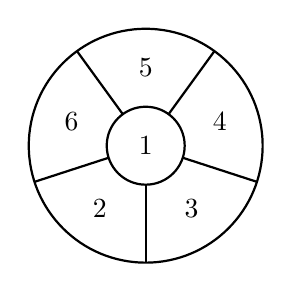
\begin{tikzpicture}[>=stealth,scale=0.9]
  \def\rIn{0.55}
  \def\rOut{1.65}
  % Circles
  \draw[thick] (0,0) circle (\rIn);
  \draw[thick] (0,0) circle (\rOut);
  
  % Radial lines
  \foreach \ang in {54, 126, 198, 270, 342} {
    \draw[thick] (\ang:\rIn) -- (\ang:\rOut);
  }
  
  % Labels
  \node at (0,0) {$1$};
  \node at (234:1.1) {$2$};
  \node at (306:1.1) {$3$};
  \node at (18:1.1) {$4$};
  \node at (90:1.1) {$5$};
  \node at (162:1.1) {$6$};
\end{tikzpicture}
